In this case, the initial voltage and SOC of the supercapacitor is set to 170V and 25.2\% respectively. The initial SOC of the battery is set at 20\%. These values are below acceptable limit. Steps similar to case 1 are also performed here. Similar to the previous case the demand of the system (44MW) exceeds the system generation capacity (40MW) between $t$ = 1s and $t$ = 2s. But unlike the previous case the ESM system provides zero $P_{stor-ref}$. This is because, the SOC of the battery and supercapacitor are low (20\% and 25.2\%) and the reference power generation by the ESM system also depends on the SOC of the battery and supercapacitor ($SOC_{Bat}$, $SOC_{SC}$) with the other two input variables, $\Delta I$ and $V_{Bus}$. Simulation results after $t$ = 2s are the same as shown in case 1.
\begin{figure}[ht!]
\begin{subfigure}{1\columnwidth}
\begin{center}
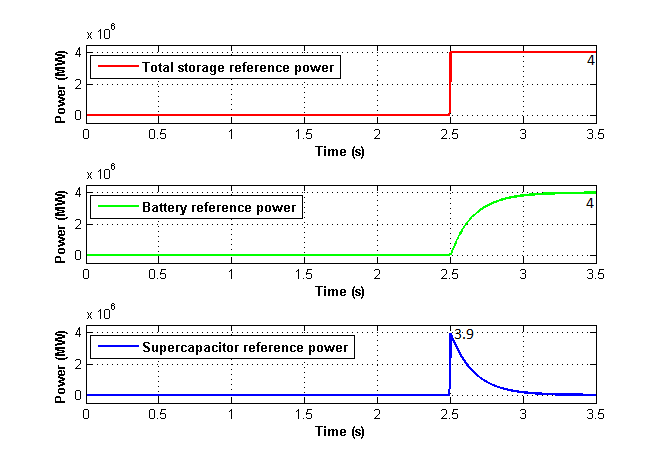
\includegraphics[height=3in, width=3.5in]{f116b}
\end{center}
\caption{Off-line simulation results.}
\label{ch5_f116b}
\end{subfigure}
\begin{subfigure}{1\columnwidth}
\begin{center}
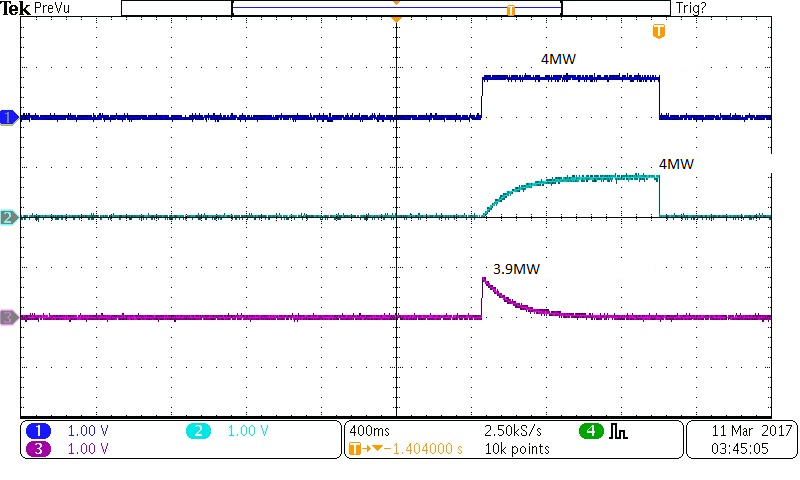
\includegraphics[height=2in, width=3.5in]{f116}
\end{center}
\caption{CHIL results-oscilloscope plots: Ch1: total storage reference power, Ch2: battery reference power, Ch3: supercapacitor reference  power (Ch1, Ch2, Ch3 = 5MW/div).}
\label{ch5_f116a}
\end{subfigure}
\caption{Reference power produced by FL controller and LPF based ESM system (case 2).}
\label{ch5_f116}
\end{figure}
